\section{Propósito y base del trabajo}

Nuestro proyecto se base en un artículo de RapGenius, cliente del proveedor
Heroku. En este artículo, RapGenius critica el reciente cambio en la política
de load-balancing de su proveedor, mostrando, con resultados de simulaciones
corridas en R, que ese cambio resulta en una pérdida de performancia
importante. Según RapGenius, una empresa necesitaría cincuenta veces más
servidores corriendo la misma aplicación para alcanzar la misma disponibilidad
con el nuevo modelo de routing, muy sencillo, que la que permitía el antiguo
modelo, que usaba un algoritmo más complicado.

\begin{figure}[h]
    \centering
    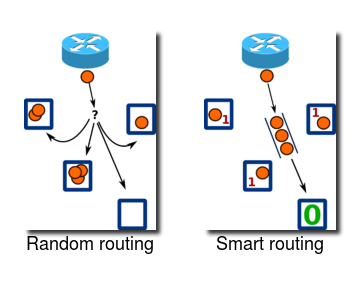
\includegraphics[height=250px]{random-smart.png}
    \caption{Los dos modelos presentados por RapGenius en su artículo}
    \label{fig:random+smart}
\end{figure}
